\chapter{Arhitektura i dizajn sustava}
		
	Arhitektura se moze podijeliti na tri podsustava:
	
	\begin{itemize}
		\item Web posluzitelj
		\item Web aplikacija
		\item Baza podataka
	\end{itemize}

	
	\textit{Web preglednik} je alat koji omogućava korisnicima pregledavanje web stranica i njihovih povezanih multimedijalnih sadržaja. Svaki internetski preglednik djeluje kao prevoditelj, jer interpretira web stranice napisane u kodu kako bi ih prikazao korisnicima na razumljiv način. Korisnici putem web preglednika šalju zahtjeve web poslužitelju.
	
	\textit{Web poslužitelj} je ključni element u radu web aplikacije. Njegova glavna uloga je olakšavanje komunikacije između klijenta i aplikacije putem HTTP protokola. Poslužitelj pokreće web aplikaciju i prenosi joj zahtjev.
	
	\textit{Web aplikacija} služi korisniku za obradu željenih zahtjeva. Aplikacija obrađuje zahtjev, pristupa bazi podataka prema potrebi i putem poslužitelja vraća korisniku odgovor u obliku HTML dokumenta koji se prikazuje u web pregledniku.
	
	\textit{Baza podataka} ima svrhu pohranjivanja i upravljanja strukturiranim podacima koji se koriste u aplikaciji. Svaki put kad korisnik šalje zahtjev putem web preglednika, web aplikacija može pristupiti bazi podataka kako bi dohvatila ili ažurirala potrebne informacije. Baza podataka omogućava učinkovit pristup, pretraživanje i manipulaciju podacima, što je ključno za pravilan rad web aplikacije.
	
	Za izradu naše web aplikacije odabrali smo programski jezik Java zajedno s Springboot radnim okvirom, kao i programski jezik JavaScript. Razvojna okruženja koja koristimo su Visual Studio Code i IntelliJ. Arhitektura sustava temelji se na MVC (Model-View-Controller) konceptu, koji je podržan od strane Springboot radnog okvira i nudi gotove predloške koji olakšavaju razvoj web aplikacije. Kao poslužitelja baze podataka smo koristili PostgreSQL.
	
	MVC koncept donosi neovisnost u razvoju pojedinih dijelova aplikacije, što olakšava testiranje, kao i dodavanje novih svojstava u sustav. Sastoji se od:
	
	\begin{itemize}
		\item \textbf{Model} - Središnja komponenta sustava koja predstavlja dinamičke strukture podataka neovisne o korisničkom sučelju. Upravlja podacima, logikom i pravilima aplikacije, te prima ulazne podatke od Controllera.
		\item \textbf{View} - Ovdje se prikazuju podaci, primjerice u obliku grafova. Moguća su različita sučelja za prikaz informacija, poput grafičkog ili tabličnog prikaza podataka.
		\item \textbf{Controller} - Prima ulaze i prilagođava ih za daljnju interakciju s Modelom ili Viewom. Upravlja korisničkim zahtjevima i temeljem njih izvodi daljnje interakcije s ostalim elementima sustava.
	\end{itemize}
		

		

				
		\section{Baza podataka}
				
				Za bazu podataka koristi se relacijska baza podataka. Svaka tablica ima svoje ime i atribute. Vrste atributa koji se mogu nalaziti u tablici su primarni ključ, strani ključ ili atribut s nekom informacijom vezanom za tablicu. Baza podataka sastoji se od tablica:
		
				\begin{packed_item}
					\item AppUser
					\item ConfirmationToken
					\item StationManager
					\item SearcherInTheField
					\item Action
					\item Station
					\item Animal
					\item PastRoutes
					\item PastLocations
					\item AnimalComment
					\item MapComment
					\item Task
				\end{packed_item}
				
				
		
			\subsection{Opis tablica}
			

				U tablici \textbf{AppUser} pohranjuju se podaci o svim korisnicima: \textit{id, userName, image, firstName, lastName, email, password, appUserRole, locked, enabled}. Primarni ključ je \textit{id}, i nema stranih ključeva. S atributom \textit{id} je u odnosu One-to-One s tablicama \textbf{StationManager} i \textbf{SearcherInTheField} i u odnosu One-to-Many s tablicama \textbf{ConfirmationToken} i \textbf{Action}.

				
				
				\begin{longtblr}[
					label=none,
					entry=none
					]{
						width = \textwidth,
						colspec={|X[6,l]|X[6, l]|X[20, l]|}, 
						rowhead = 1,
					} %definicija širine tablice, širine stupaca, poravnanje i broja redaka naslova tablice
					\hline \SetCell[c=3]{c}{\textbf{AppUser}}	 \\ \hline[3pt]
					\SetCell{LightGreen}id & BIGINT	&  	id korisnika 	\\ \hline
					userName	& VARCHAR &  korisničko ime 	\\ \hline 
					image & BYTEA &  heksadekatski zapis korisničke slike  \\ \hline 
					firstName & VARCHAR	&  ime korisnika  \\ \hline 
					lastName & VARCHAR	&  prezime korisnika  \\ \hline 
					email & VARCHAR	&  email korisnika  \\ \hline 
					password & VARCHAR	&  lozinka korisnika  \\ \hline
					appUserRole & VARCHAR	&  uloga korisnika  \\ \hline 
					locked & BOOLEAN & je li korisnika potvrdio admin \\ \hline
					enabled & BOOLEAN & je li korisnik potvrđen emailom \\ \hline
				\end{longtblr}
				
				U tablici \textbf{ConfirmationToken} pohranjuju se podaci za token za potvrdu poslanu korisniku: \textit{id, token, createdAt, expiresAt, confirmedAt, user}. Svaki token je povezan s korisnikom kojem je poslan preko \textit{user} u koji se sprema id korisnika. Primarni ključ je \textit{id}, a strani ključ je \textit{user}. S atributom \textit{user} je u odnosu Many-to-One s tablicom \textbf{AppUser}.
				
				\begin{longtblr}[
					label=none,
					entry=none
					]{
						width = \textwidth,
						colspec={|X[6,l]|X[6, l]|X[20, l]|}, 
						rowhead = 1,
					} %definicija širine tablice, širine stupaca, poravnanje i broja redaka naslova tablice
					\hline \SetCell[c=3]{c}{\textbf{ConfirmationToken}}	 \\ \hline[3pt]
					\SetCell{LightGreen}id & BIGINT	&  	id tokena 	\\ \hline
					token & VARCHAR & token \\ \hline
					createdAt & TIMESTAMP & vrijeme kada je token stvoren \\ \hline
					expiersAt & TIMESTAMP & vrijeme kada token ističe \\ \hline
					confirmedAt & TIMESTAMP & vrijeme kada je token potvrđen \\ \hline
					\SetCell{LightBlue}user	& BIGINT &  id korisnika kojemu je poslan token \\ \hline  
				\end{longtblr}

				U tablici \textbf{StationManager} pohranjuju se dodatni podaci za voditelja postaje: \textit{stationManagerId, userId, stationId}. Primarni ključ  je \textit{stationManagerId}, te su \textit{userId } i \textit{stationId }  su strani ključevi. S atributom \textit{userId } je u odnosu One-to-One s tablicom \textbf{AppUser}, s atributom \textit{stationManagerId} je u odnosu Many-to-One s tablicom \textbf{Station}.

				
				\begin{longtblr}[
					label=none,
					entry=none
					]{
						width = \textwidth,
						colspec={|X[6,l]|X[6, l]|X[20, l]|}, 
						rowhead = 1,
					} %definicija širine tablice, širine stupaca, poravnanje i broja redaka naslova tablice

					\hline \SetCell[c=3]{c}{\textbf{StationManager}}	 \\ \hline[3pt]
					\SetCell{LightGreen}id & BIGINT	&  	id korisničkog računa voditelja 	\\ \hline
					\SetCell{LightBlue}stationId  & BIGINT	&  	id postaje koju vodi voditelj 	\\ \hline
					\SetCell{LightBlue}userId  & BIGINT	&  id usera	\\ \hline
				\end{longtblr}
			

			U tablici \textbf{SearcherInTheField} primarni ključ je \textit{searcherInTheFieldId}. Strani ključevi su \textit{stationId}, \textit{userId} i \textit{actionId}. S atributom \textit{userId} je u odnosu One-to-One s tablicom \textbf{AppUser}, s atributom \textit{stationId} je u odnosu Many-to-One s tablicom \textbf{Station}, s atributom \textit{actionId} je u odnosu Many-to-One s tablicom \textbf{Action}.

			
				\begin{longtblr}[
					label=none,
					entry=none
					]{
						width = \textwidth,
						colspec={|X[10,l]|X[6, l]|X[20, l]|}, 
						rowhead = 1,
					} %definicija širine tablice, širine stupaca, poravnanje i broja redaka naslova tablice
					\hline \SetCell[c=3]{c}{\textbf{SearcherInTheField}}	 \\ \hline[3pt]
					\SetCell{LightGreen}searcherInTheFieldId & BIGINT	&  	id korisničkog računa tragača 	\\ \hline
					\SetCell{LightBlue}stationId & BIGINT	&  	id postaje kojoj pripada 	\\ \hline
					\SetCell{LightBlue} userId  & BIGINT	&  id usera	\\ \hline
					 qualification	& VARCHAR & osposobljenosti tragača 	\\ \hline  
					 currentPosition & JSON &  trenutna pozicija tragača	\\ \hline 
					\SetCell{LightBlue} actionId  & BIGINT	&  id akcije na kojoj tragač sudjeluje	\\ \hline
				\end{longtblr}
			

			U tablici \textbf{Action} pohranjuju se podaci vezani uz određenu akciju. Primarni ključ je \textit{actionId}, a strani ključ je \textit{appUserId}. S atributom \textit{appUserId} je u odnosu Many-to-One s tablicom \textbf{AppUser} i s atributom \textit{stationId} je u odnosu One-to-One s tablicom \textbf{Station}.


			
			\begin{longtblr}[
				label=none,
				entry=none
				]{
					width = \textwidth,
					colspec={|X[8,l]|X[6, l]|X[20, l]|}, 
					rowhead = 1,
				} %definicija širine tablice, širine stupaca, poravnanje i broja redaka naslova tablice
				
				\hline \SetCell[c=3]{c}{\textbf{Action}}	 \\ \hline[3pt]
				\SetCell{LightGreen}  actionId & BIGINT	&  	id akcije 	\\ \hline
				\SetCell{LightBlue}appUserId & BIGINT	&  	id korisnika (istraživača) koji je započeo akciju 	\\ \hline
				\SetCell{LightBlue} stationId & BIGINT	& id postaje kojoj se posalo zahtjev za tragačima \\ \hline
				actionName	& TEXT &  naziv akcije 	\\ \hline
				actionType & TEXT &  tip akcije	\\ \hline  
				locationName & TEXT &  ime lokacije na kojoj se odvija akcija (npr. Biokovo)	\\ \hline 
				mapViewCriteria & JSON & odabrani kriteriji (od strane istraživača) za prikaz životinja na mapi \\ \hline
				qualificationsJson & JSON & popis traženih kvalifikacija tragača na akciji \\ \hline
			\end{longtblr}
			

			U tablici \textbf{Station} pohranjuju se podaci vezani uz postaju. Primarni ključ je \textit{stationId}. Strani ključ je \textit{stationId}. S atributom \textit{stationId} je u odnosu Many-to-One s tablicom \textbf{Station}.
			
			\begin{longtblr}[
				label=none,
				entry=none
				]{
					width = \textwidth,
					colspec={|X[8,l]|X[6, l]|X[20, l]|}, 
					rowhead = 1,
				} %definicija širine tablice, širine stupaca, poravnanje i broja redaka naslova tablice

				\hline \SetCell[c=3]{c}{\textbf{Station}}	 \\ \hline[3pt]
				\SetCell{LightGreen}stationId & BIGINT	&  	id postaje 	\\ \hline
				stationName & VARCHAR & ime postaje \\ \hline
				coordinatesJson & JSON & popis koordinata postaje te koordinata za prikaz područje pokrivanja za određeno osposobljenje \\ \hline
			\end{longtblr}
			
			U tablici \textbf{Animal} o svim životinjama za određenu postaju. Primarni ključ je \textit{animalId} nema stranih ključeva. S atributom \textit{id} je u odnosu One-to-Many s tablicom \textbf{Location}.

			\begin{longtblr}[
				label=none,
				entry=none
				]{
					width = \textwidth,
					colspec={|X[7,l]|X[6, l]|X[20, l]|}, 
					rowhead = 1,
				} %definicija širine tablice, širine stupaca, poravnanje i broja redaka naslova tablice

				\hline \SetCell[c=3]{c}{\textbf{Animal}}	 \\ \hline[3pt]
				\SetCell{LightGreen} animalId & BIGINT	&  	id životinje 	\\ \hline
				name & VARCHAR & ime životinje \\ \hline
				breed & VARCHAR & vrsta životinje \\ \hline
				description & VARCHAR & opis životinje \\ \hline
				image & BYTEA & slika životinje \\ \hline
				currentPosition & JSON & trenutna pozicija životinje\\ \hline
				\SetCell{LightBlue}stationId & BIGINT	&  id postaje, odn. područja (npr. postaja Biokovo) kojoj životinja pripada \\ \hline
			\end{longtblr}
			

			U tablici \textbf{PastRoutes} pohranjuju se podaci o svim prijašnjim rutama kojima je istraživač prošao na određenoj akciji. Primarni ključ je \textit{pastRoutesId}, a strani ključevi su \textit{actionId} i \textit{searcherId}. S atributom \textit{actionId} je u odnosu Many-to-One s tablicom \textbf{Action}, a s atributom \textit{searcherId} je u odnosu Many-to-One s tablicom \textbf{SearcherInTheField} .

			\begin{longtblr}[
				label=none,
				entry=none
				]{
					width = \textwidth,
					colspec={|X[8,l]|X[6, l]|X[20, l]|}, 
					rowhead = 1,
				} %definicija širine tablice, širine stupaca, poravnanje i broja redaka naslova tablice

				\hline \SetCell[c=3]{c}{\textbf{PastRoutes}}	 \\ \hline[3pt]
				\SetCell{LightGreen}pastRoutesId & BIGINT & id rute \\ \hline
				routeWaypoints & JSON & koordinate rute\\ \hline
				\SetCell{LightBlue}actionId & BIGINT	&  id akcije na kojoj je istraživač prošo tom rutom \\ \hline
				\SetCell{LightBlue}searcherId & BIGINT	&  id istraživača čija je ruta zabilježena  \\ \hline
				
			\end{longtblr}
			
			U tablici \textbf{PastLocations} pohranjuju se podaci o svim prijašnjim lokacijama životinja ili istraživača na određenoj akciji. Primarni ključ je \textit{pastLocationId}, a strani ključevi su \textit{actionId}, \textit{animalId} i \textit{searcherId}. S atributom \textit{actionId} je u odnosu Many-to-One s tablicom \textbf{Action}, s atributom \textit{animalId} je u odnosu Many-to-One s tablicom \textbf{Animal}, a s atributom \textit{searcherId} je u odnosu Many-to-One s tablicom \textbf{SearcherInTheField} .
			
			\begin{longtblr}[
				label=none,
				entry=none
				]{
					width = \textwidth,
					colspec={|X[9,l]|X[6, l]|X[20, l]|}, 
					rowhead = 1,
				} %definicija širine tablice, širine stupaca, poravnanje i broja redaka naslova tablice
				
				\hline \SetCell[c=3]{c}{\textbf{PastLocations}}	 \\ \hline[3pt]
				\SetCell{LightGreen}pastLocationId & BIGINT & id lokacije \\ \hline
				positionCoordinates & JSON & koordinate lokacije\\ \hline
				\SetCell{LightBlue}actionId & BIGINT	&  id akcije tokom koje je zabilježena lokacija \\ \hline
				\SetCell{LightBlue}searcherId & BIGINT	&  id istraživača čija je lokacija zabilježenja  \\ \hline
				\SetCell{LightBlue}animalId & BIGINT	&  id životinje čija je prijašnja lokacija zabilježenja  \\ \hline
				
			\end{longtblr}		
			
			U tablici \textbf{AnimalComment} pohranjuju se svi komentari koji su ostavljeni životinji na određenoj akciji. Primarni ključ je \textit{animalCommentId}, a strani ključevi su \textit{actionId} i \textit{animalId}. S atributom \textit{actionId} je u odnosu Many-to-One s tablicom \textbf{Action}, te s atributom \textit{animalId} je u odnosu Many-to-One s tablicom \textbf{Animal}.
			
			\begin{longtblr}[
				label=none,
				entry=none
				]{
					width = \textwidth,
					colspec={|X[9,l]|X[6, l]|X[20, l]|}, 
					rowhead = 1,
				} %definicija širine tablice, širine stupaca, poravnanje i broja redaka naslova tablice
				
				\hline \SetCell[c=3]{c}{\textbf{AnimalComment}}	 \\ \hline[3pt]
				\SetCell{LightGreen}animalCommentId & BIGINT & id komentara \\ \hline
				comment & VARCHAR & komentar ostavljen životinji\\ \hline
				userName & VARCHAR & korisničko ime korisnika koji je ostavio komentar životinji lokacije\\ \hline
				\SetCell{LightBlue}actionId & BIGINT	&  id akcije tokom koje je zabilježena lokacija \\ \hline
				\SetCell{LightBlue}animalId & BIGINT	&  id životinje čija je prijašnja lokacija zabilježenja  \\ \hline
			\end{longtblr}
			
			U tablici \textbf{MapComment} pohranjuju se svi komentari koji su ostavljeni na mapi na određenoj akciji. Primarni ključ je \textit{mapCommentId}, a strani ključ je \textit{actionId}. S atributom \textit{actionId} je u odnosu Many-to-One s tablicom \textbf{Action}.
			
			\begin{longtblr}[
				label=none,
				entry=none
				]{
					width = \textwidth,
					colspec={|X[9,l]|X[6, l]|X[20, l]|}, 
					rowhead = 1,
				} %definicija širine tablice, širine stupaca, poravnanje i broja redaka naslova tablice
				
				\hline \SetCell[c=3]{c}{\textbf{MapComment}}	 \\ \hline[3pt]
				\SetCell{LightGreen}mapCommentId & BIGINT & id komentara \\ \hline
				comment & VARCHAR & komentar ostavljen životinji\\ \hline
				userName & VARCHAR & korisničko ime korisnika koji je ostavio komentar životinji lokacije\\ \hline
				positionCoordinates & JSON & koordinate lokacije gdje je na mapi ostavljen komentar\\ \hline
				\SetCell{LightBlue}actionId & BIGINT	&  id akcije tokom koje je zabilježena lokacija \\ \hline
			\end{longtblr}
			
			U tablici \textbf{Task} pohranjuju se podaci zadataka koji su dodjeljeni tragaču na određenoj akciji. Primarni ključ je \textit{taskId}, strani ključevi su \textit{actionId} i \textit{searcher}. S atributom \textit{actionId} je u odnosu Many-to-One s tablicom \textbf{Action}, a s atributom \textit{searcherId} je u odnosu Many-to-One s tablicom \textbf{SearcherInTheField}.
			
			\begin{longtblr}[
				label=none,
				entry=none
				]{
					width = \textwidth,
					colspec={|X[9,l]|X[6, l]|X[20, l]|}, 
					rowhead = 1,
				} %definicija širine tablice, širine stupaca, poravnanje i broja redaka naslova tablice
				
				\hline \SetCell[c=3]{c}{\textbf{Task}}	 \\ \hline[3pt]
				\SetCell{LightGreen}taskId & BIGINT & id zadatka \\ \hline
				taskComment	& VARCHAR &  komentar za zadatak od strane istra	\\ \hline 
				taskToDo	& VARCHAR &  opis  što tragač mora napraviti 	\\ \hline 
				completed & BOOLEAN & je li zadatak završen ili ne \\ \hline
				routeWaypoints & JSON & koordinate rute koju tragač treba proći na zadatku\\ \hline
				\SetCell{LightBlue}searcherId & BIGINT	&  id istraživača čija je lokacija zabilježenja  \\ \hline
				\SetCell{LightBlue}actionId & BIGINT	&  	id akcije kojoj pripada zahtjev 	\\ \hline
			\end{longtblr}
			
			\subsection{Dijagram baze podataka}
				\begin{figure}[H]
					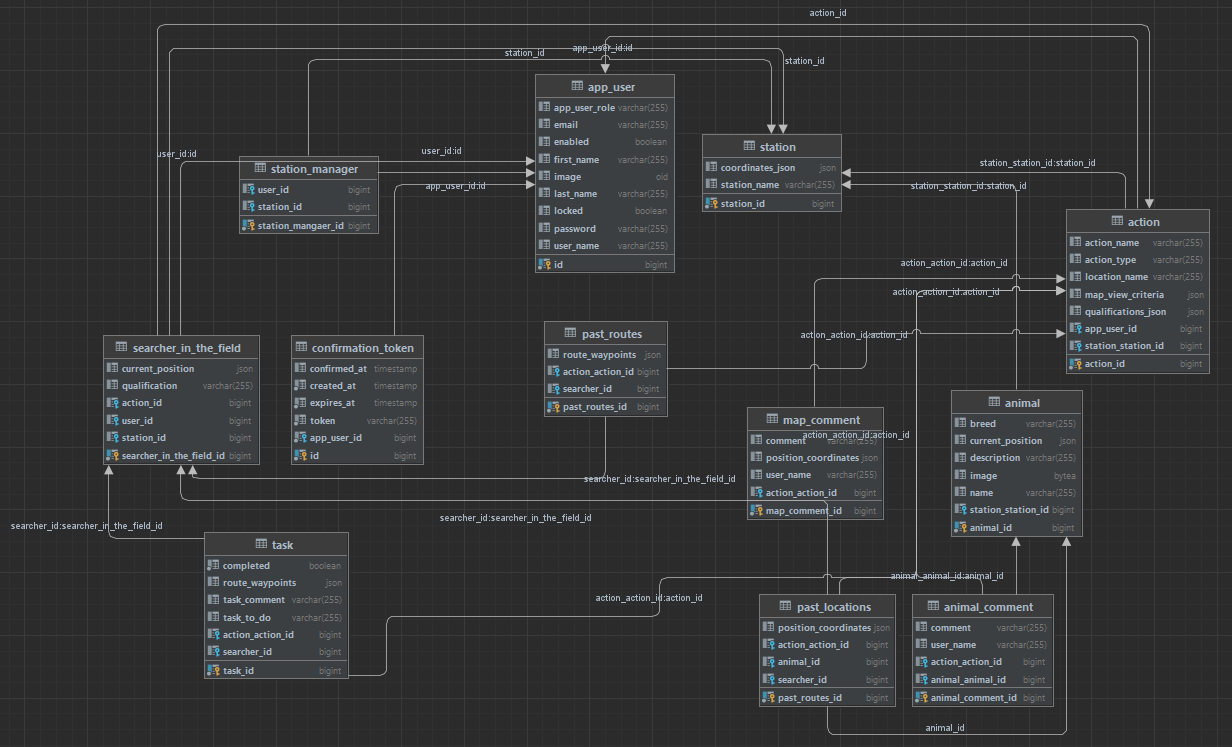
\includegraphics[scale=0.6]{dijagrami/dijagramBaza.png}
					\centering
					\caption{Dijagram baze podataka}
					\label{fig:promjene}
				\end{figure}
			\eject
			
			
		\section{Dijagram razreda}
		Dijagram razreda podijeljen je zbog bolje preglednosti na tri dijela: Controllers, Models i DTO. Prikazane su veze koje ostvaruju razredi unutar istog dijela dijagrama, a odnosi između razreda u različitim dijelovima mogu se zaključiti iz tipova atributa. Metode korištene u Controller razredima vraćaju \textit{ResponseEntity}, koji predstavlja HTTP odgovor, ili samo kod odgovora HTTP-a. U svom radu koriste objekte za prijenos podataka (DTO) i ostvaruju komunikaciju s klijentskom stranom.
			
			\begin{figure}[H]
				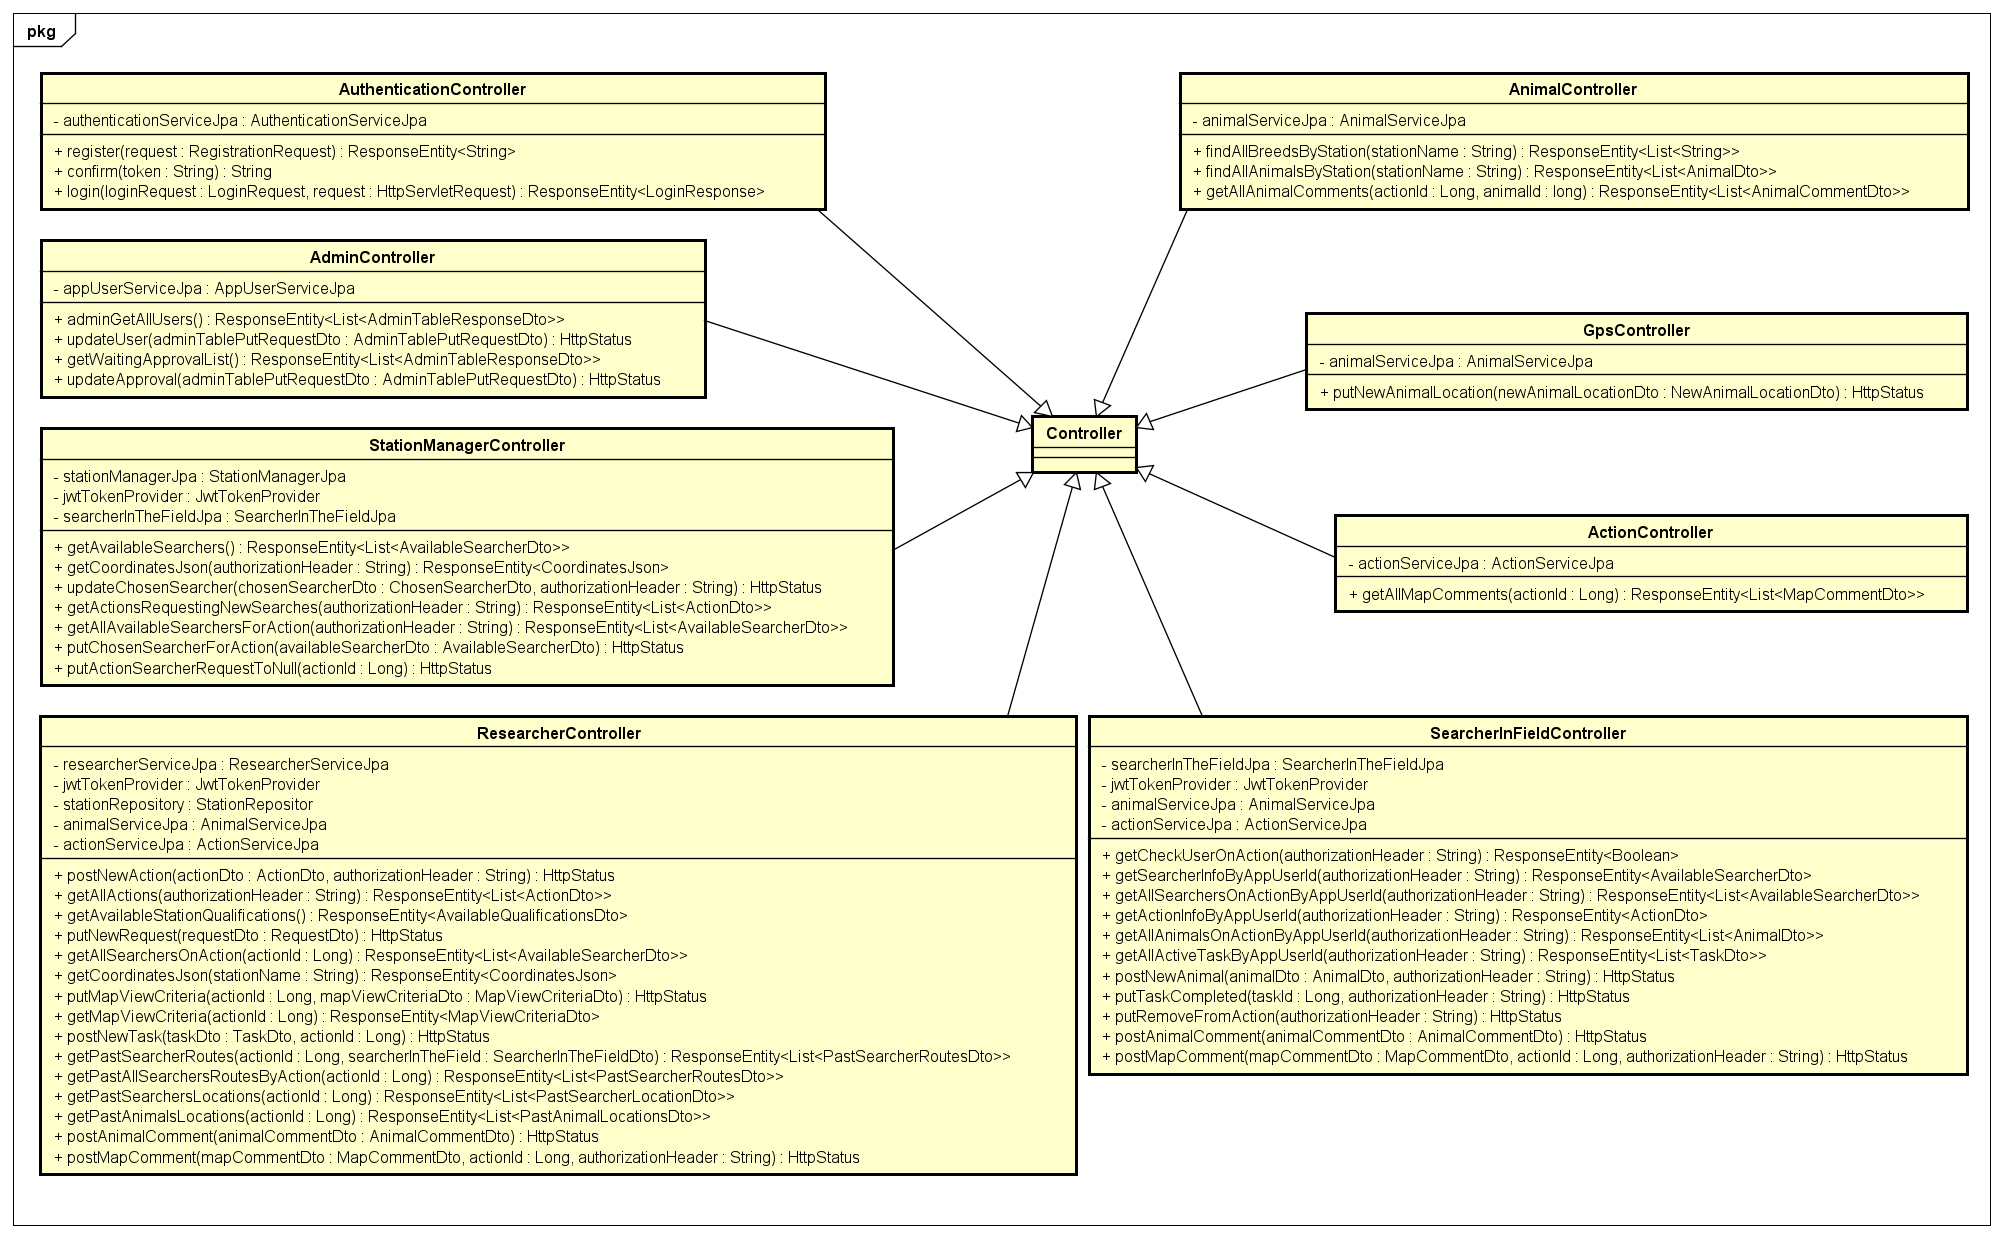
\includegraphics[scale=0.5]{dijagrami/Controllers.png} 
				\centering
				\caption{Dijagram razreda - dio Controllers}
				\label{fig:promjene}
			\end{figure}
			
			\begin{figure}[H]
				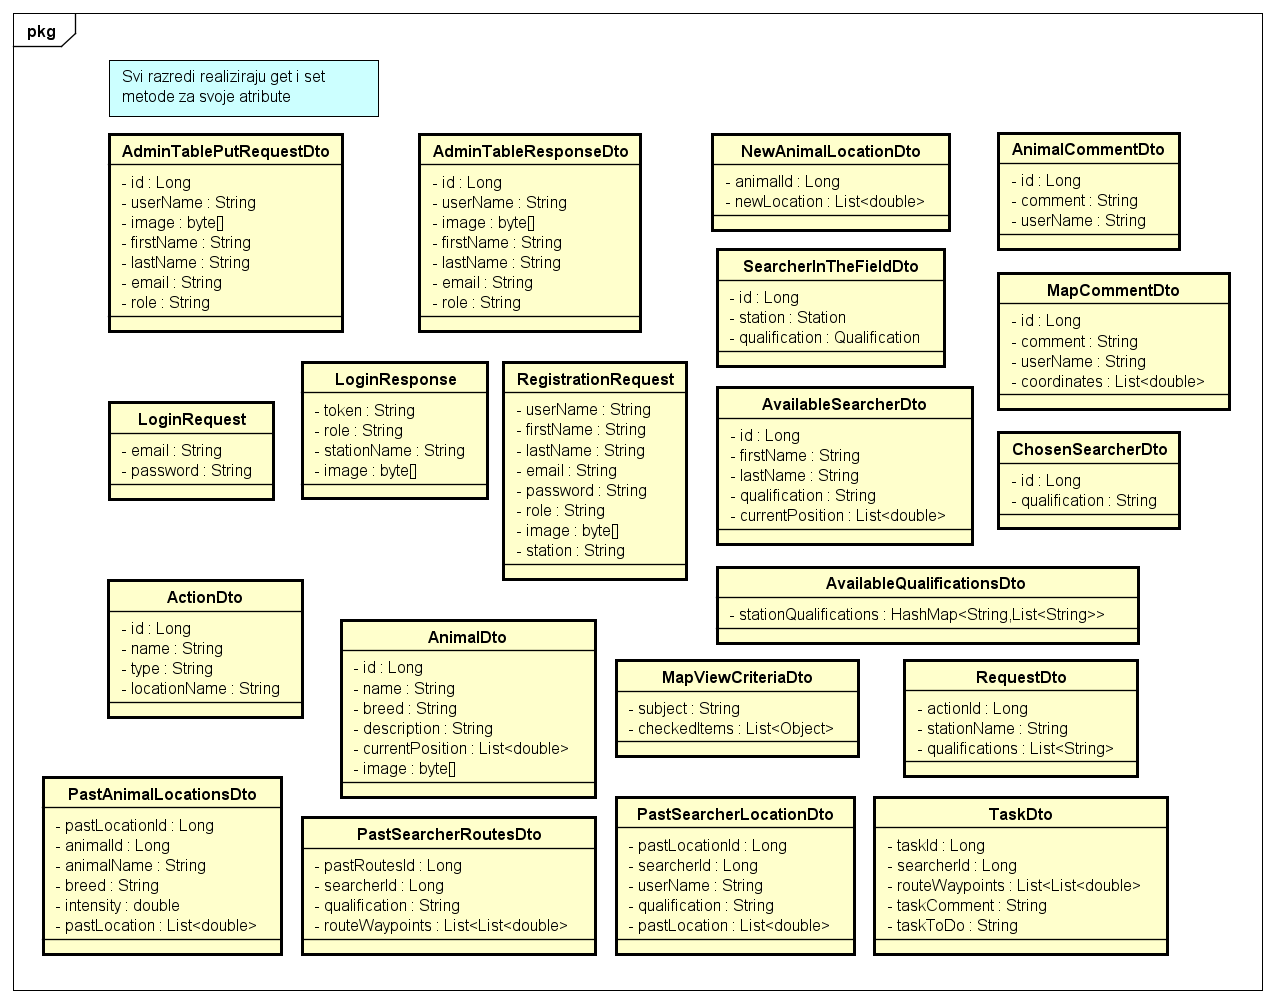
\includegraphics[scale=0.5]{dijagrami/DTO.png} 
				\centering
				\caption{Dijagram razreda - dio DTO}
				\label{fig:promjene}
			\end{figure}
			
			\begin{figure}[H]
				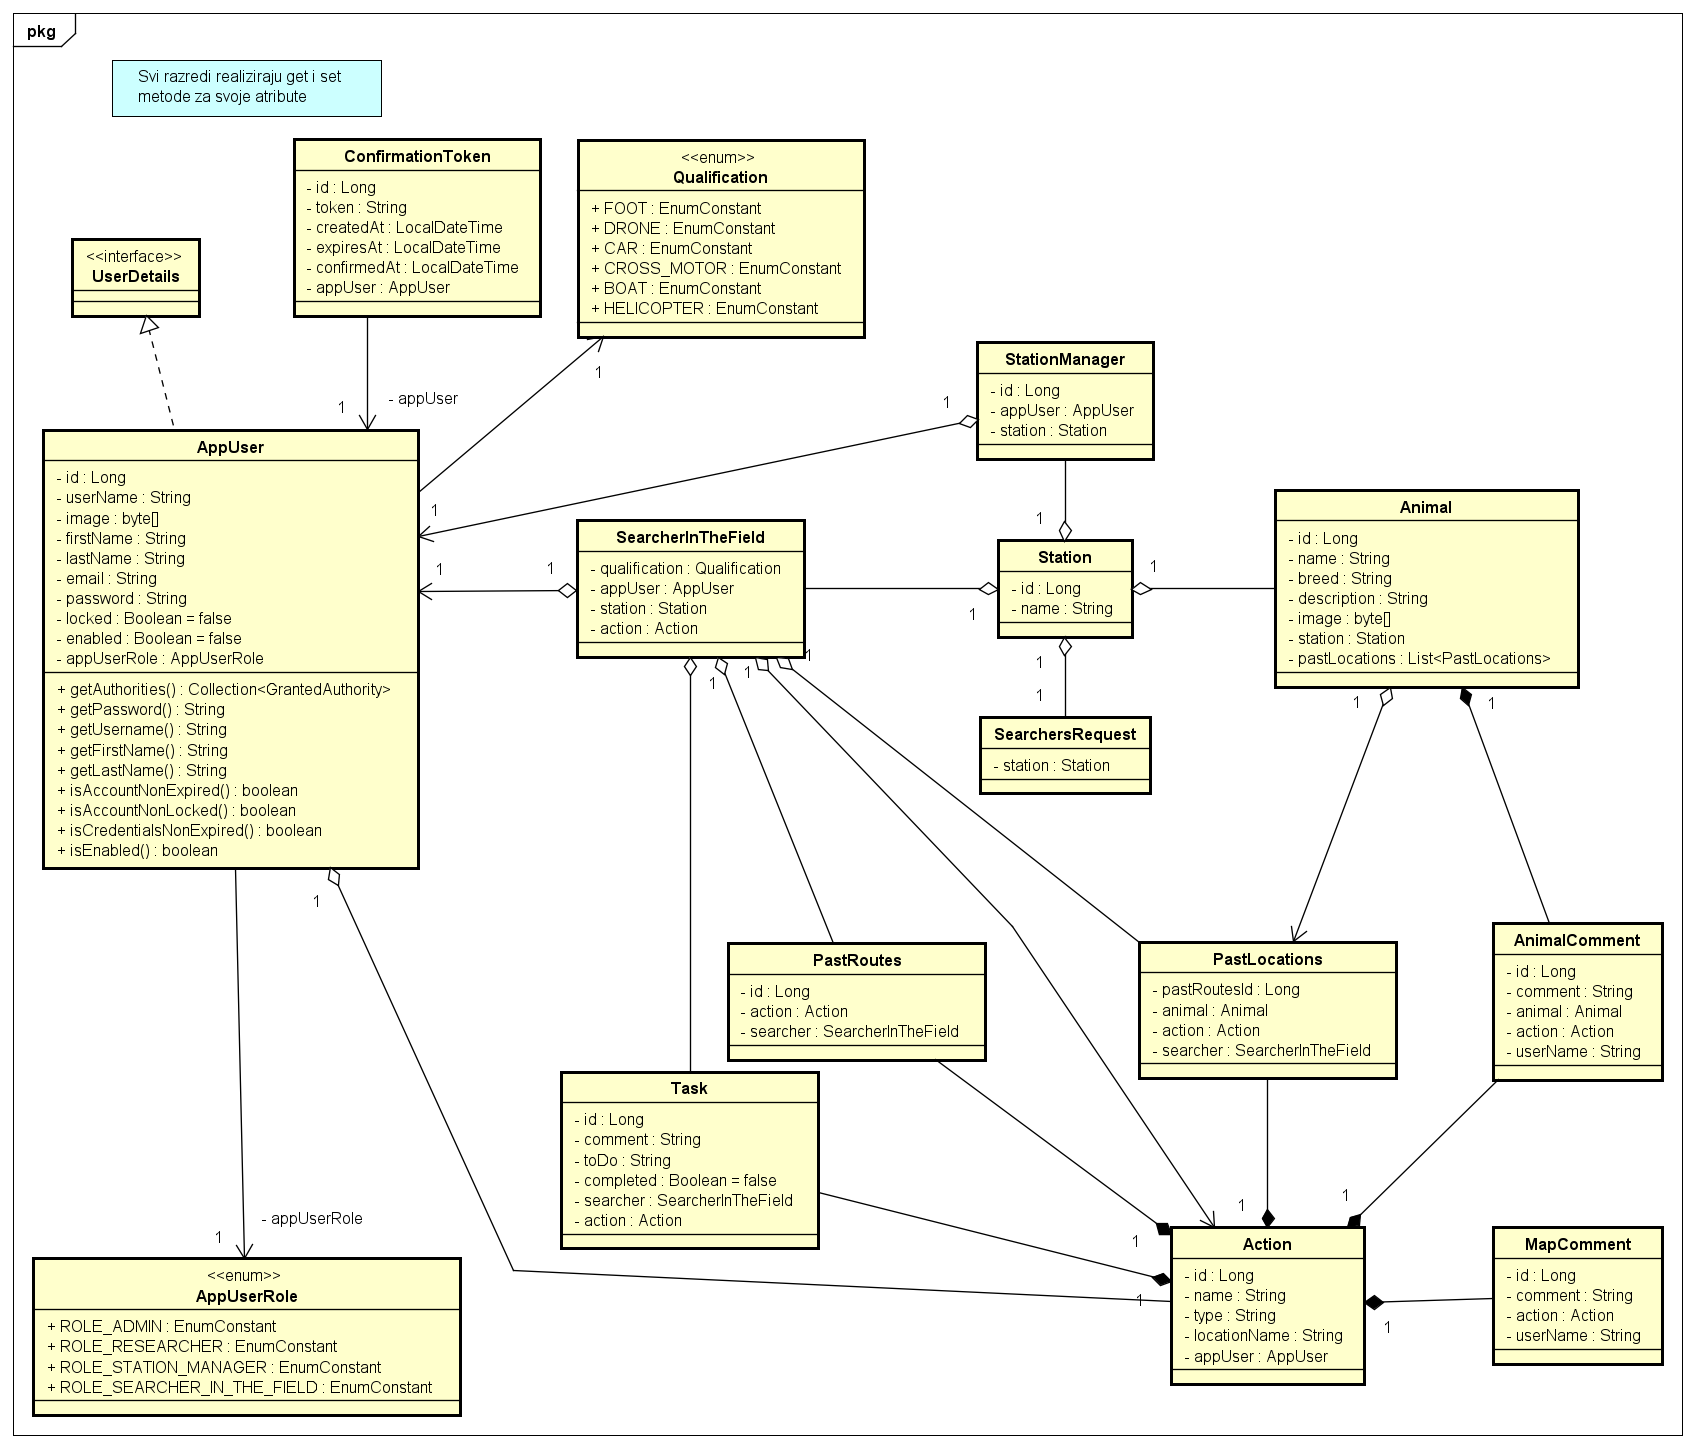
\includegraphics[scale=0.4]{dijagrami/Model.png} 
				\centering
				\caption{Dijagram razreda - dio Models}
				\label{fig:promjene}
			\end{figure}
			
			
			\eject
		
		\section{Dijagram stanja}
			
			
			Dijagrami stanja prikazuju kako sustav prelazi iz jednog stanja u drugo kao odgovor na događaje. Prijavljenom korisniku, u ovom slučaju istraživaču, prikazuje se početna stranica s nekoliko opcija: pregled vlastitih akcija, stvaranje nove akcije i pregled osobnih podataka. Nakon odabira opcije stvaranja nove akcije, korisniku se nudi mogućnost slanja zahtjeva za tragačima za pripadajuću akciju. U slučaju da nema slobodnih tragača, sustav obavijesti korisnika i čeka na idući zahtjev. Ako se istraživaču dodijele tragači, može im dodijeliti zadatke. Zatim ima opciju unosa komentara na zadatak. Odabirom opcije ,,Moje akcije“ , istraživač može vidjeti sve svoje akcije i pregledati njihove članove te završiti neku od akcija.  Također, istraživač može odabrati prikaz karte i urediti je po želji. Nakon toga može ostaviti komentar na karti.
			
			\begin{figure}[H]
				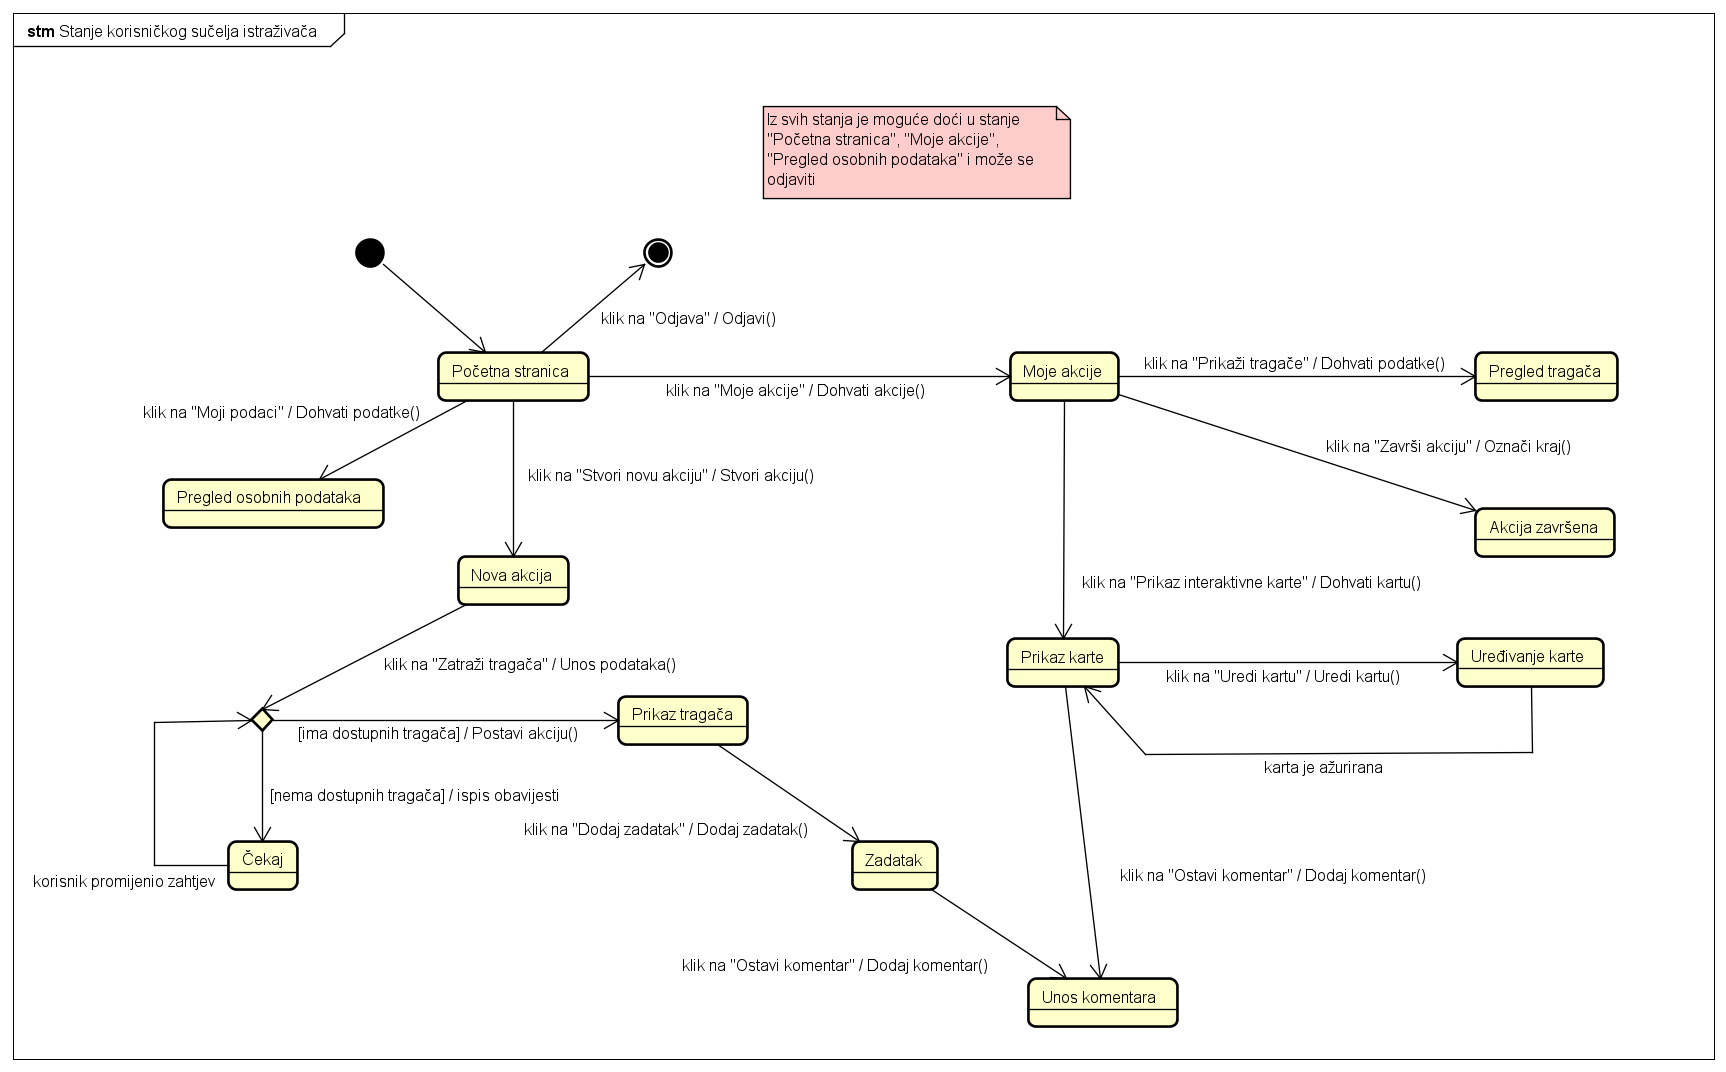
\includegraphics[scale=0.3]{dijagrami/DijagramStanja.png} 
				\centering
				\caption{Dijagram stanja}
				\label{fig:promjene}
			\end{figure}
			
			
			\eject 
		
		\section{Dijagram aktivnosti}
			
			Dijagrami aktivnosti upotrebljavaju se za modeliranje dinamičkog ponašanja sustava. Izvođenje aktivnosti prikazano je kroz niz akcija koje čine upravljačke tokove i tokove objekata. Prikazan je proces stvaranja nove akcije. Aktivnost započinje prijavom istraživača u sustav. Nakon uspješne prijave, istraživaču se prikazuje početna stranica. Odabirom opcije za stvaranje nove akcije aplikacija prikazuje formu za unos podataka o akciji. Istraživač unosi podatke o akciji, a sustav ih pohranjuje u bazu podataka. Zatim istraživač šalje zahtjev za tragačima, a aplikacija prikazuje formu za unos detalja o zahtjevu. Aplikacija prosljeđuje zahtjev voditelju postaje koji dodjeljuje tragače akciji (pretpostavlja se da ima dostupnih tragača). Popis tragača se pohranjuje u bazu i prikazuje u aplikaciji. Na zahtjev za dodjeljivanje zadatka nekom od tragača prikazuje se forma za unos zadatka. Zadatak se sprema u bazu podataka, a istraživač može unijeti i komentar o zadatku. Nakon završetka unosa svih podataka o akciji aplikacija prikazuje poruku da su svi podaci spremljeni i aktivnost završava.
			
			\begin{figure}[H]
				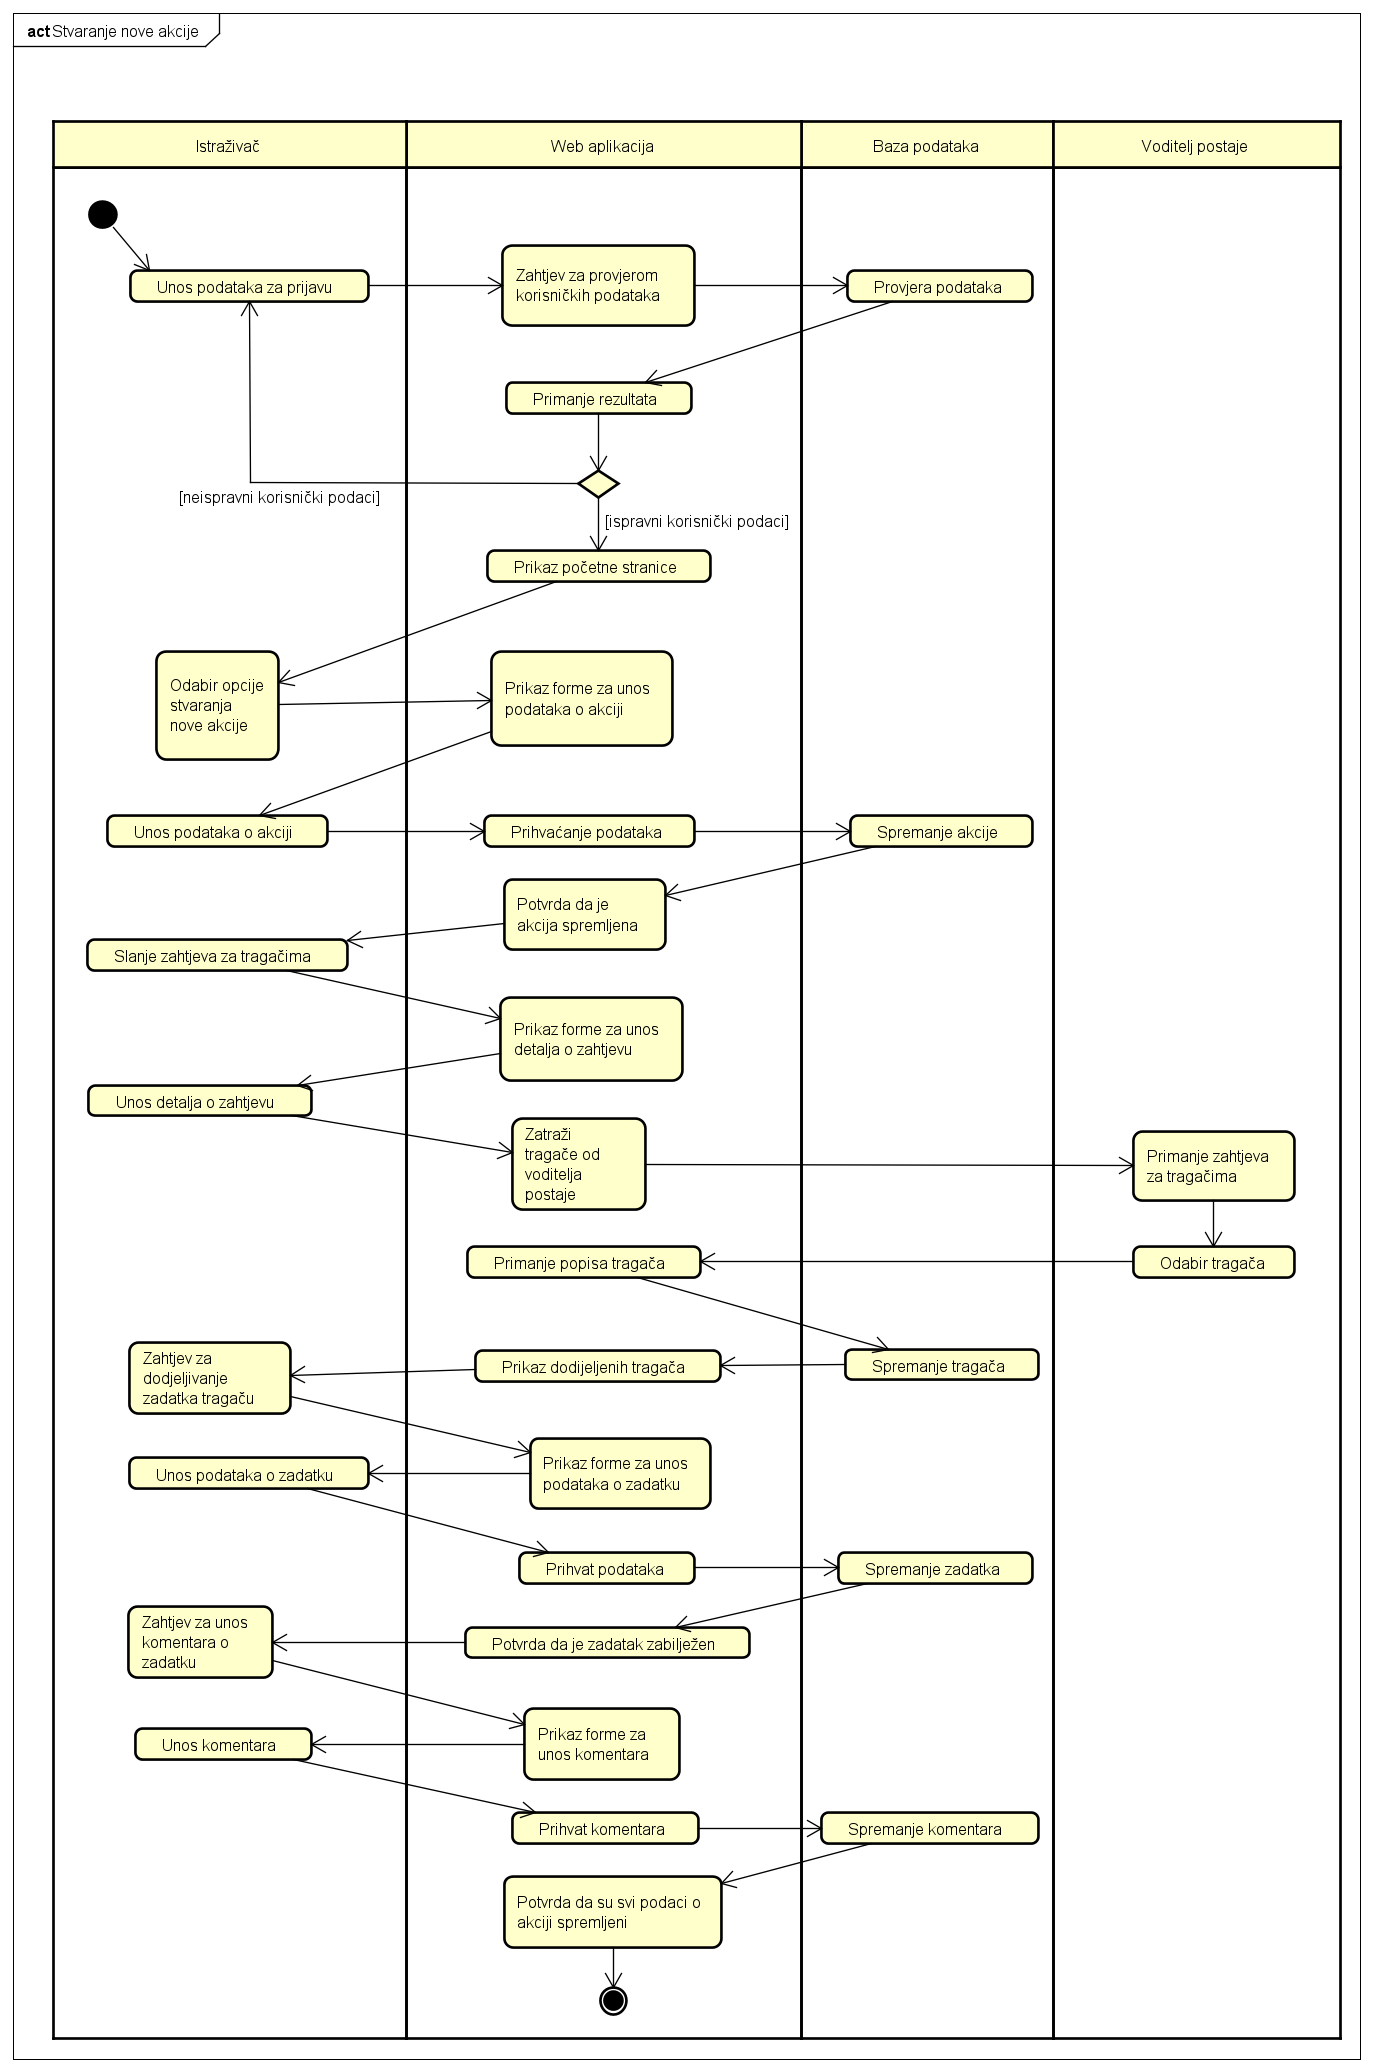
\includegraphics[scale=0.4]{dijagrami/DijagramAkt.png} 
				\centering
				\caption{Dijagram aktivnosti}
				\label{fig:promjene}
			\end{figure}
			
			\eject
		\section{Dijagram komponenti}
		
			 Dijagram komponenti prikazuje komponente u sustavu i njihovu organizaciju. Sustav se sastoji od tri glavne komponente: \textbf{Frontend web aplikacije}, \textbf{Backend web aplikacije} i \textbf{Baza podataka}. \textbf{Frontend web aplikacije} sastoji se od manjih komponenti: \textbf{ApiService.js, index.js, Admin, Assets, General, Login, Manager, Register, Researcher, Searcher}. Komponenta \textbf{ApiService.js} služi za komunikaciju s backendom pomoću HTTP metoda \textit{get, post, put, delete}. Komponente \textbf{Admin, Assets, General, Login, Manager, Register, Researcher, Searcher} su skupovi react komponenti koji služe za prikaz za određenu svrhu. Npr. \textbf{Admin} ima komponente koje se prikazuju samo za admina, a \textbf{Manager} ima komponente koje se pokazuju samo za voditelja postaje. \textbf{Backend web aplikacije} sastoji se od komponenti \textbf{Controller, Service, Mapper, DTO, Repository}. \textbf{Controller} prima i odgovara na HTTP metode i poziva usluge u komponenti \textbf{Service}. Komponenta \textbf{Service} obavlja funkcije aplikacije, npr. registracija korisnika, dodavanje komentara, stvaranje postaje itd. Komponenta \textbf{Repository} služi za komunikaciju s \textbf{Bazom podataka}. \textbf{DTO} sadrži objekte s podacima koji se koriste u aplikaciji. \textbf{Mapper} služi za pretvorbu objekata iz \textbf{DTO} u normalne objekte, npr. pretvorbu AnimalDto u Animal.
			 
			 
			 \begin{figure}[H]
			 	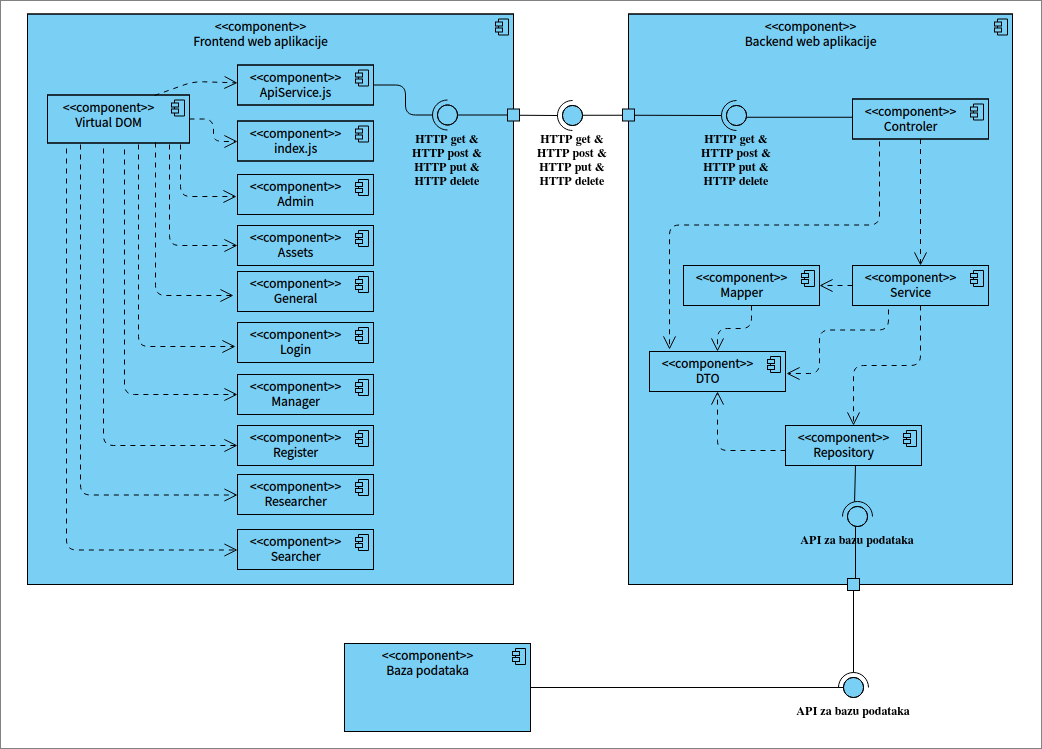
\includegraphics[scale=0.45]{dijagrami/dijagram_komponenti2.png}
			 	\centering
			 	\caption{Dijagram komponenti}
			 	\label{fig:promjene}
			 \end{figure}